
% Start and ice-breaker:

% Introducing myself



\begin{frame}{Introducing Myself}
   \begin{block}{Education}
    \begin{itemize}
     \item Master's Degrees in Microelectronics and Mathematics
     \item Doctoral Degree in Microelectronics
     \item Home University: TU Wien
    \end{itemize}

   \vspace*{-2cm}
   \begin{flushright}
     
\includegraphics[width=0.15\textwidth]{figures/TU-Signet}
   \end{flushright}

   \end{block}



   \begin{block}{Interests}
    \begin{itemize}
     \item Efficient Numerics on Modern Hardware
     \item High-level APIs
     \item Semiconductor Device Simulation
    \end{itemize}

   \end{block}

   \begin{block}{Contact}
    \begin{itemize}
     \item Email: rupp@mcs.anl.gov
     \item Web: http://www.karlrupp.net/
     \item Find me at: Google+, Twitter, LinkedIn
    \end{itemize}
   \end{block}

\end{frame}






\begin{frame}{Before we start...}

   \begin{block}{Goal of this Workshop}
    \begin{itemize}
     \item {\Huge \textbf{\color{red} You}} should learn new things about HPC
    \end{itemize}
   \end{block}

   \vspace*{1cm}
   \begin{block}{Ask Questions}
    \begin{itemize}
     \item Tell me if you do not understand
     \item Ask for further details
     \item Don't be shy
    \end{itemize}
   \end{block}

\end{frame}




%%%%%% General PETSc information %%%%%%%%%%

%%% What is PETSc

%
% Stats, Who, Philosophy
%




\section{PETSc Overview}
\begin{frame}{PETSc}
   \begin{center} \Large \textbf{About PETSc} \end{center}
\end{frame}

\begin{frame}[fragile]
\frametitle{PETSc Origins}
 
 \begin{center} \LARGE
  \definecolor{ddviolet}{rgb}{0.561, 0.067, 0.455}  % RGB 143-17-116
  PETSc was developed as a Platform for \\[0.2em] \textbf{\color{ddviolet} Experimentation}
 \end{center}

 \vspace{1cm}
 \begin{block}{We want to experiment with different}
 \begin{itemize}
  \item Models
  \item Discretizations
  \item Solvers
  \item Algorithms
 \end{itemize}
 \end{block}

 \begin{block}{These boundaries are often blurred...}
 \end{block}

 \begin{flushright}
  \vspace*{-5cm}
  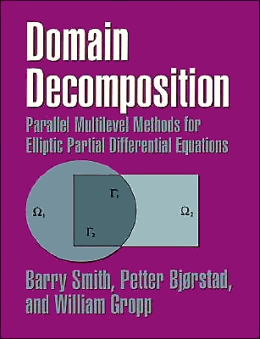
\includegraphics[width=0.4\textwidth]{dd-book-smith.png}
 \end{flushright}

\end{frame}




\newcommand\ganttline[4]{% line, tag, start end
   \node at (0,#1/2+.1) [anchor=base east] {#2};
   \fill[blue] (#3/\xtick-1991/\xtick,#1/2-.1) rectangle (#4/\xtick-1991/\xtick,#1/2+.1);}
\newcommand\ganttlabel[6]{% year, label, color, yloc, anchor
  \node[#3] at (#1/\xtick+#6/\xtick-1991/\xtick,#4) [anchor=#5] {#2};
  \fill[#3] (#1/\xtick-1991/\xtick,1/2-.1) rectangle (#1/\xtick-1991/\xtick+0.04,15/2+.1);}

\begin{frame}{Timeline}
%\frame{
\begin{figure}[htbp]
\vspace*{-0.4cm}
\hspace*{-0.8cm}
\def\present{2016.2}
\def\xtick{2.8}
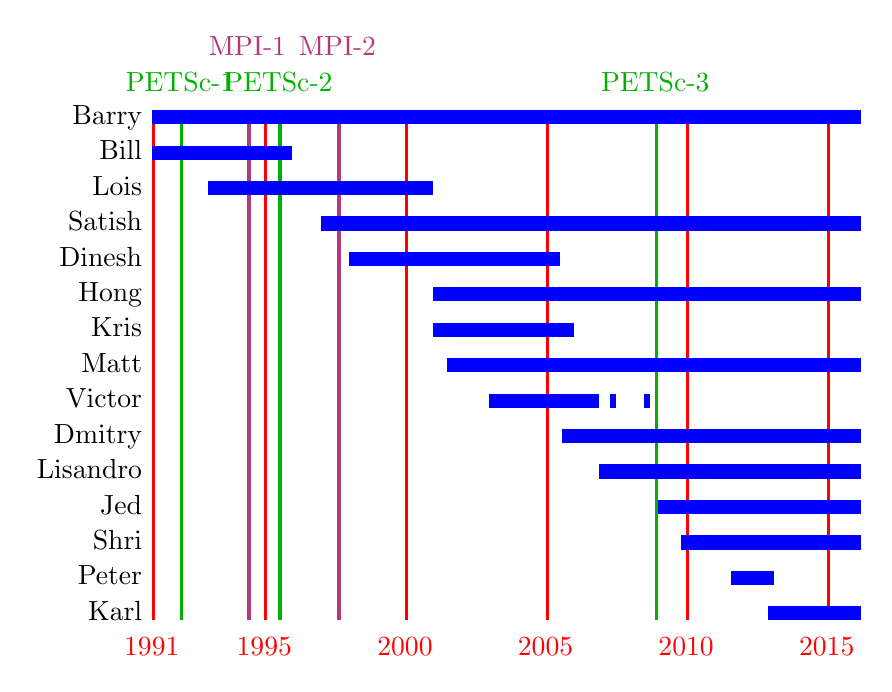
\begin{tikzpicture}[y=-0.9cm]
   %\draw[help lines] (0.5,5) grid (8,0.5);
   \ganttlabel{1991}{1991}{red}{7.7}{north}{0}
   \ganttlabel{1995}{1995}{red}{7.7}{north}{0}
   \ganttlabel{2000}{2000}{red}{7.7}{north}{0}
   \ganttlabel{2005}{2005}{red}{7.7}{north}{0}
   \ganttlabel{2010}{2010}{red}{7.7}{north}{0}
   \ganttlabel{2015}{2015}{red}{7.7}{north}{0}
   \ganttlabel{1992}{PETSc-1}{green!70!black}{0}{center}{0}
   \ganttlabel{1994.4}{MPI-1}{magenta!70!black}{-.5}{center}{0}
   \ganttlabel{1997.6}{MPI-2}{magenta!70!black}{-.5}{center}{0}
   \ganttlabel{1995.5}{PETSc-2}{green!70!black}{0}{center}{0}
   \ganttlabel{2008.9}{PETSc-3}{green!70!black}{0}{center}{0}
   \ganttline{1}{Barry}{1991}{\present}
   \ganttline{2}{Bill}{1991}{1996}
   \ganttline{3}{Lois}{1993}{2001}
   \ganttline{4}{Satish}{1997}{\present}
   \ganttline{5}{Dinesh}{1998}{2005.5}
   \ganttline{6}{Hong}{2001}{\present}
   \ganttline{7}{Kris}{2001}{2006}
   \ganttline{8}{Matt}{2001.5}{\present}
   \ganttline{9}{Victor}{2003}{2006.9}
   \ganttline{9}{}{2007.3}{2007.5}
   \ganttline{9}{}{2008.5}{2008.7}
   \ganttline{10}{Dmitry}{2005.6}{\present}
   \ganttline{11}{Lisandro}{2006.9}{\present}
   \ganttline{12}{Jed}{2009}{\present}
   \ganttline{13}{Shri}{2009.8}{\present}
   \ganttline{14}{Peter}{2011.6}{2013.12}
   \ganttline{15}{Karl}{2012.9}{\present}
\end{tikzpicture}
\end{figure}
%}
\end{frame}

\begin{frame}{PETSc}
\vspace*{-0.2cm}
\begin{center} {\bf Portable} Extensible Toolkit for Scientific Computing \end{center}
\vspace*{-0.2cm}
\begin{block}{Architecture}
    \begin{itemize}  \vspace*{-0.2cm}
    \item tightly coupled (e.g. XT5, BG/P, Earth Simulator)
    \item loosely coupled such as network of workstations
    \item GPU clusters (many vector and sparse matrix kernels)
    \end{itemize}
\end{block} \vspace*{-0.2cm}

\begin{block}{Software Environment}
  \begin{itemize}\vspace*{-0.2cm}
   \item Operating systems (Linux, Mac, Windows, BSD, proprietary Unix)
   \item Any compiler
   \item Usable from C, C++, Fortran 77/90, Python, and MATLAB
   \item Real/complex, single/double/quad precision, 32/64-bit int
  \end{itemize}
\end{block}\vspace*{-0.2cm}

\begin{block}{System Size}
  \begin{itemize}\vspace*{-0.2cm}
   \item 500B unknowns, 75\% weak scalability on Jaguar (225k cores) \\
    and Jugene (295k cores)
   \item Same code runs performantly on a laptop
  \end{itemize}
\end{block}\vspace*{-0.2cm}


\begin{block}{Free to everyone (BSD-style license), open development}\end{block} \vspace*{-0.4cm}

\end{frame}


\begin{frame}{PETSc}

\begin{center}Portable {\bf Extensible} Toolkit for Scientific Computing \end{center}

\begin{block}{Philosophy: Everything has a plugin architecture}
\begin{itemize}
  \item Vectors, Matrices, Coloring/ordering/partitioning algorithms
  \item Preconditioners, Krylov accelerators
  \item Nonlinear solvers, Time integrators
  \item Spatial discretizations/topology$^*$
\end{itemize}

\end{block}

\begin{block}{Example}
  \begin{itemize}
   \item Vendor supplies matrix format and associated preconditioner, distributes
	compiled shared library.  
   \item Application user loads plugin at runtime, no source
	code in sight.
  \end{itemize}
\end{block}

 \vspace{2cm}
\end{frame}


\begin{frame}{PETSc}

\begin{center} Portable Extensible {\bf Toolkit} for Scientific Computing \end{center}

\begin{block}{Toolset}
  \begin{itemize}
   \item algorithms
   \item (parallel) debugging aids
   \item low-overhead profiling
  \end{itemize}
\end{block}

\begin{block}{Composability}
 \begin{itemize}
  \item try new algorithms by choosing from product space
  \item composing existing algorithms (multilevel, domain decomposition, splitting)
 \end{itemize}
\end{block}

\begin{block}{Experimentation}
\begin{itemize}
  \item Impossible to pick the solver \emph{a priori}
  \item PETSc's response: expose an algebra of composition
  \item keep solvers decoupled from physics and discretization
\end{itemize}
\end{block}
\end{frame}

\begin{frame}{PETSc}
\vspace*{-0.2cm}
\begin{center}
 Portable Extensible Toolkit for {\bf Scientific Computing}
\end{center}
\vspace*{-0.2cm}

  \begin{block}{Computational Scientists}
    \begin{itemize}\vspace*{-0.2cm}
    \item PyLith (CIG), Underworld (Monash), Magma Dynamics (LDEO, Columbia), PFLOTRAN (DOE), SHARP/UNIC (DOE)
    \end{itemize}
  \end{block}\vspace*{-0.2cm}
  
  \begin{block}{ Algorithm Developers (iterative methods and preconditioning)} \end{block}\vspace*{-0.4cm}
  
  \begin{block}{ Package Developers}
    \begin{itemize} \vspace*{-0.2cm}
    \item SLEPc, TAO, Deal.II, Libmesh, FEniCS, PETSc-FEM, MagPar, OOFEM, FreeCFD, OpenFVM
    \end{itemize}
  \end{block}\vspace*{-0.2cm}
  
  \begin{block}{Funding}
    \begin{itemize} \vspace*{-0.2cm}    
      \item Department of Energy
      \begin{itemize}\item SciDAC, ASCR ISICLES, MICS Program, INL Reactor Program
      \end{itemize}
    \item National Science Foundation
      \begin{itemize}\item CIG, CISE, Multidisciplinary Challenge Program
      \end{itemize}
    \end{itemize}
  \end{block}\vspace*{-0.2cm}
  
  \begin{block}{Documentation and Support}
   \begin{itemize}\vspace*{-0.2cm}
    \item Hundreds of tutorial-style examples
    \item Hyperlinked manual, examples, and manual pages for all routines
    \item Support from \url{petsc-maint@mcs.anl.gov}
   \end{itemize}
  \end{block}
  
\end{frame}

\begin{frame}[fragile]

\frametitle{The Role of PETSc}

\vspace*{\fill}
\begin{minipage}{\linewidth}
\begin{quote}
\Large Developing parallel, nontrivial PDE solvers that deliver high performance is still difficult and requires
months (or even years) of concentrated effort.

\medskip

PETSc is a toolkit that can ease these difficulties and reduce the development time, but it is not a black-box PDE
solver, nor a \color{blue}{silver bullet}.
\end{quote}
\qquad --- Barry Smith
\end{minipage}
\vspace*{\fill}\vspace*{\fill}

\end{frame}



\begin{frame}[fragile]

\frametitle{The Role of PETSc}

\vspace*{\fill}
\begin{minipage}{\linewidth}
\begin{quote}
\Large You want to think about how you decompose your data
structures, how you think about them globally. [...] 

\medskip

If you
were building a house, you'd start with a set of blueprints
that give you a picture of what the whole house looks
like. You wouldn’t start with a bunch of tiles and say.
``Well I'll put this tile down on the ground, and then I'll
find a tile to go next to it.''

\medskip

But all too many people try to
build their parallel programs by creating the smallest
possible tiles and then trying to have the structure of
their code emerge from the chaos of all these little
pieces. You have to have an organizing principle if
you're going to survive making your code parallel.

\end{quote}

\qquad --- Bill Gropp

\qquad --- http://www.rce-cast.com/Podcast/rce-28-mpich2.html
\end{minipage}
\vspace*{\fill}\vspace*{\fill}

\end{frame}


%\begin{frame}{PETSc}
%   \begin{center} \Large \textbf{First Steps} \end{center}
%\end{frame}




\begin{frame}[fragile]
\frametitle{PETSc}
 \begin{block}{Obtaining PETSc}
 \begin{itemize}
  \item Linux Package Managers
  \item Web: http://mcs.anl.gov/petsc, download tarball
  \item Git: https://bitbucket.org/petsc/petsc
  \item Mercurial: https://bitbucket.org/petsc/petsc-hg
 \end{itemize}
 \end{block}

 \begin{block}{Installing PETSc}
 \begin{itemize}
  \item
 \begin{lstlisting}[escapechar={@}]
$> cd /path/to/petsc/workdir
$> git clone \
     https:@/@/bitbucket.org/petsc/petsc.git \
     --branch master --depth 1
$> cd petsc
 \end{lstlisting}
  \item
 \begin{lstlisting}
$> export PETSC_DIR=$PWD PETSC_ARCH=mpich-gcc-dbg
$> ./configure --with-cc=gcc --with-fc=gfortran 
                 --download-f-blas-lapack
                 --download-{mpich,ml,hypre}
\end{lstlisting}
 \end{itemize}
 \end{block}

\end{frame}


\begin{frame}[fragile]
\frametitle{PETSc External Packages}

\begin{block}{Most packages can be automatically}
  \begin{itemize}  \vspace*{-0.2cm}
    \item Downloaded
    \item Configured and Built (in \lstinline|$PETSC_DIR/externalpackages|)
    \item Installed with PETSc
  \end{itemize}
\end{block} \vspace*{-0.2cm}
  
\begin{block}{Currently works for}
  \begin{itemize}  \vspace*{-0.2cm}
    \item petsc4py
    \item PETSc documentation utilities (Sowing, lgrind, c2html)
    \item BLAS, LAPACK, BLACS, ScaLAPACK, PLAPACK
    \item MPICH, MPE, OpenMPI
    \item ParMetis, Chaco, Jostle, Party, Scotch, Zoltan
    \item MUMPS, Spooles, SuperLU, SuperLU\_Dist, UMFPack, pARMS
    \item PaStiX, BLOPEX, FFTW, SPRNG
    \item Prometheus, HYPRE, ML, SPAI
    \item Sundials
    \item Triangle, TetGen, FIAT, FFC, Generator
    \item HDF5, Boost
  \end{itemize}
\end{block}

\end{frame}



\begin{frame}[fragile]
\frametitle{PETSc Pyramid}
 \begin{block}{PETSc Structure} \vspace{0.3cm}
   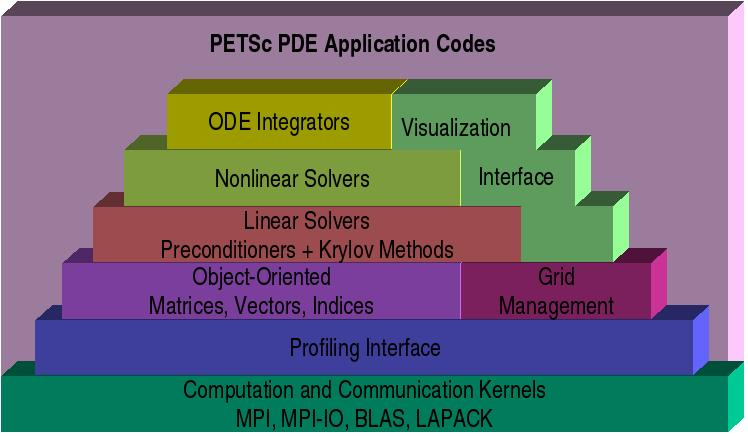
\includegraphics[width=1.0\textwidth]{PETScPyramid.jpg}
 \end{block}

\end{frame}

\begin{frame}[fragile]
\frametitle{Flow Control for a PETSc Application}

\begin{center}
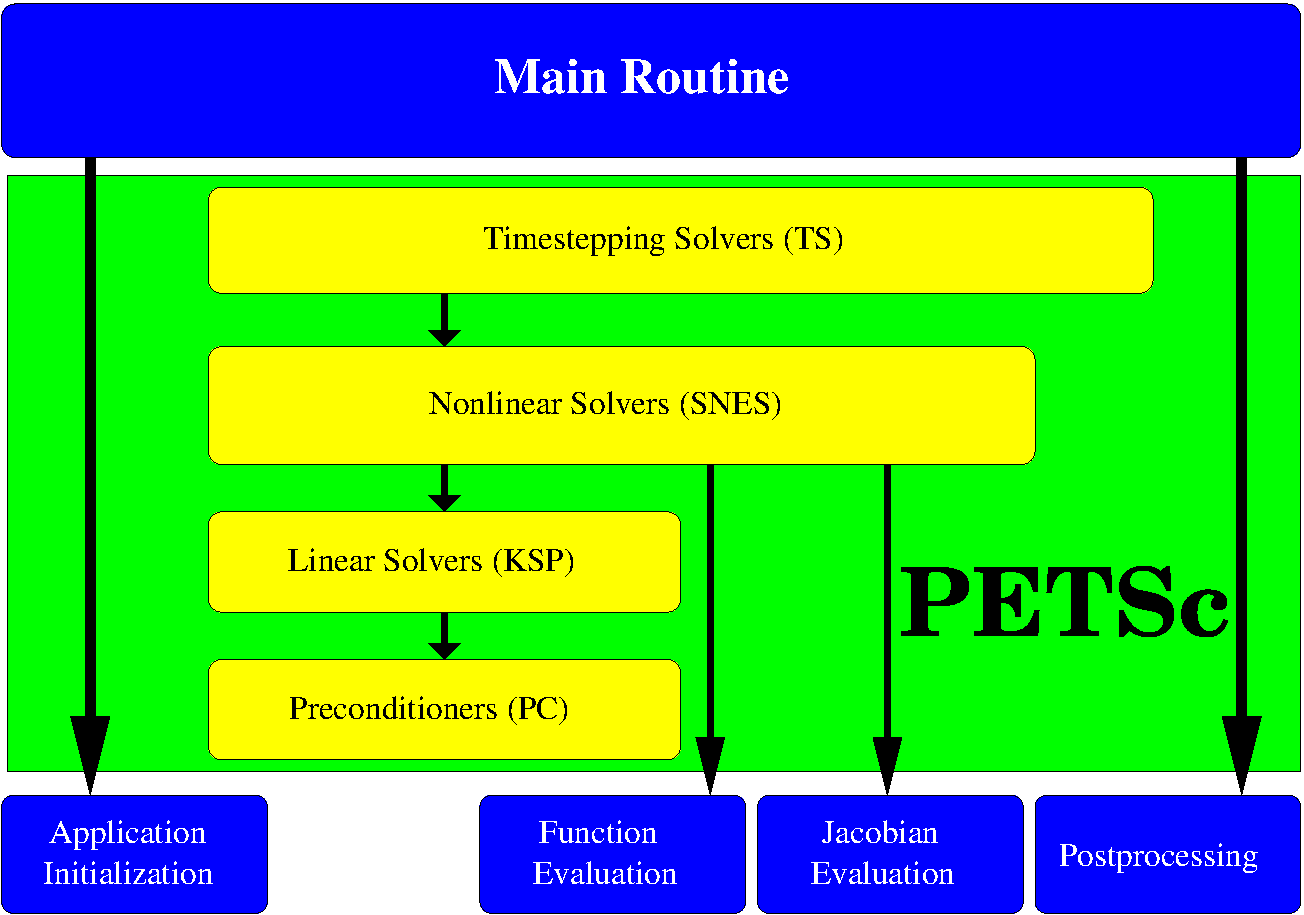
\includegraphics[width=4.0in]{figures/FlowControl}
\end{center}
\end{frame}



\begin{frame}[fragile]
\frametitle{PETSc Objects}
\begin{block}{Sample Code}
  \begin{lstlisting}
    Mat A;
    PetscInt m,n,M,N;
    MatCreate(comm,&A);
    MatSetSizes(A,m,n,M,N);      /* or PETSC_DECIDE */ 
    MatSetOptionsPrefix(A,"foo_");
    MatSetFromOptions(A);
    /* Use A */
    MatView(A,PETSC_VIEWER_DRAW_WORLD);
    MatDestroy(A);
  \end{lstlisting}
  \end{block}
  
  \begin{block}{Remarks}
  \begin{itemize}
  \item \lstinline|Mat| is an opaque object (pointer to incomplete type)
    \begin{itemize}
     \item Assignment, comparison, etc, are cheap
    \end{itemize}
  \item What's up with this ``Options'' stuff?
    \begin{itemize}
    \item We will discuss this later...
    \end{itemize}
  \end{itemize}
  
\end{block}
\end{frame}

\begin{frame}{Basic PetscObject Usage}

\begin{block}{Every object in PETSc supports a basic interface}
\vspace{0.3cm}
\begin{tabular}{|r|l|}
\hline
Function & Operation \\
\hline
\texttt{Create()}               & create the object \\
\texttt{Get/SetName()}          & name the object \\
\texttt{Get/SetType()}          & set the implementation type \\
\texttt{Get/SetOptionsPrefix()} & set the prefix for all options \\
\texttt{SetFromOptions()}       & customize object from command line \\
\texttt{SetUp()}                & perform other initialization \\
\texttt{View()}                 & view the object \\
\texttt{Destroy()}              & cleanup object allocation \\
\hline
\end{tabular}

\end{block}

\begin{block}{Also, all objects support the \lstinline|-help| option.}\end{block}

\end{frame}


\begin{frame}[fragile]{PETSc Options}
\begin{block}{Ways to set options}
  \begin{itemize}
  \item Command line
  \item Filename in the third argument of \lstinline|PetscInitialize()|
  \item \lstinline|~/.petscrc|
  \item \lstinline|$PWD/.petscrc|
  \item \lstinline|$PWD/petscrc|
  \item \lstinline|PetscOptionsInsertFile()|
  \item \lstinline|PetscOptionsInsertString()|
  \item \lstinline|PETSC_OPTIONS| environment variable
  \item command line option \lstinline|-options_file [file]|
  \end{itemize}
\end{block}
\end{frame}


\begin{frame}[fragile]{PETSc Options}

\begin{block}{Example of Command Line Control}
  %\lstinline|$> cd $PETSC_DIR/src/snes/examples/tutorials && make ex5}| \\
  \begin{itemize}
  \item \lstinline|$> ./ex5 -da_grid_x 10 -da_grid_y 10 -par 6.7| \\
      \lstinline|       -snes_monitor -{ksp,snes}_converged_reason| \\
      \lstinline|       -snes_view|
  \item \lstinline|$> ./ex5 -da_grid_x 10 -da_grid_y 10 -par 6.7| \\
      \lstinline|       -snes_monitor -{ksp,snes}_converged_reason| \\
      \lstinline|       -snes_view -mat_view_draw -draw_pause 0.5|
  \item \lstinline|$> ./ex5 -da_grid_x 10 -da_grid_y 10 -par 6.7| \\
      \lstinline|       -snes_monitor -{ksp,snes}_converged_reason| \\
      \lstinline|       -snes_view -mat_view_draw -draw_pause 0.5| \\
      \lstinline|       -pc_type lu -pc_factor_mat_ordering_type natural|
  \item Use \lstinline|-help| to find other ordering types
\end{itemize}
\end{block}
\end{frame}



\section{Application Integration}
\begin{frame}{PETSc}
   \begin{center} \Large \textbf{Application Integration} \end{center}
\end{frame}

\begin{frame}{Application Integration}

\begin{block}{Be willing to experiment with algorithms}
  \begin{itemize}
    \item No optimality without interplay between physics and algorithmics
  \end{itemize}
\end{block}

\begin{block}{Adopt flexible, extensible programming}
  \begin{itemize}
    \item Algorithms and data structures not hardwired
  \end{itemize}
\end{block}

\begin{block}{Be willing to play with the real code}
  \begin{itemize}
    \item Toy models have limited usefulness
    \item But make test cases that run quickly
  \end{itemize}
\end{block}

\begin{block}{If possible, profile before integration}
  \begin{itemize}
    \item Automatic in PETSc
  \end{itemize}
\end{block}

\end{frame}

\begin{frame}[fragile]{Incorporating PETSc into Existing Codes}
  \begin{block}{PETSc does not seize \lstinline|main()|, does not control output}   \end{block} \vspace*{-0.4cm}
  %\pause
  \begin{block}{Propogates errors from underlying packages, flexible}   \end{block} \vspace*{-0.4cm}
  %\pause
  \begin{block}{Nothing special about \lstinline|MPI_COMM_WORLD|}   \end{block} \vspace*{-0.4cm}
  %\pause
  \begin{block}{Can wrap existing data structures/algorithms}
    \begin{itemize} \vspace*{-0.2cm}
    \item \lstinline|MatShell|, \lstinline|PCShell|, full implementations
    \item \lstinline|VecCreateMPIWithArray()|
    \item \lstinline|MatCreateSeqAIJWithArrays()|
    \item Use an existing semi-implicit solver as a preconditioner
    \item Usually worthwhile to use native PETSc data structures \\
      unless you have a good reason not to
    \end{itemize}
  \end{block} \vspace*{-0.4cm}
  %\pause
  \begin{block}{Uniform interfaces across languages}
    \begin{itemize} \vspace*{-0.2cm}
    \item C, C++, Fortran 77/90, Python, MATLAB
    \end{itemize}
  \end{block} \vspace*{-0.4cm}
  %\pause
  \begin{block}{Do not have to use high level interfaces (e.g.~SNES, TS, DM)}
    \begin{itemize} \vspace*{-0.2cm}
    \item but PETSc can offer more if you do, like MFFD and SNES Test
    \end{itemize}
  \end{block}
\end{frame}

\begin{frame}{Integration Stages}

\begin{block}{\color{red} Version Control}
  \begin{itemize} \vspace*{-0.1cm}
    \item It is impossible to overemphasize
  \end{itemize} \vspace*{-0.1cm}
\end{block}

\begin{block}{Initialization}
  \begin{itemize} \vspace*{-0.1cm}
    \item Linking to PETSc
  \end{itemize} \vspace*{-0.1cm}
\end{block}

\begin{block}{Profiling}
  \begin{itemize} \vspace*{-0.1cm}
    \item Profile {\color{red} before} changing
    \item Also incorporate command line processing
  \end{itemize} \vspace*{-0.1cm}
\end{block}

\begin{block}{Linear Algebra}
  \begin{itemize} \vspace*{-0.1cm}
    \item First PETSc data structures
  \end{itemize} \vspace*{-0.1cm}
\end{block}

\begin{block}{Solvers}
  \begin{itemize} \vspace*{-0.1cm}
    \item Very easy after linear algebra is integrated
  \end{itemize}
\end{block}

\end{frame}




%%%%%%%%%%%%%%%%%%%%%%%%%%%%

\section{PETSc and Accelerators}
\begin{frame}{PETSc}
   \begin{center} \Large \textbf{PETSc and Accelerators} \end{center}
\end{frame}




\begin{frame}{Typical PETSc Operations}
 
  \begin{block}{``Sparse'' Linear Algebra}
   \begin{itemize}
    \item Sparse Matrix-Vector Operations (on-node)
    \item Vector Operations (on and across nodes)
    \item Only on small patches: Dense Operations (\emph{small} matrices)
   \end{itemize}
  \end{block}

   \begin{center}
     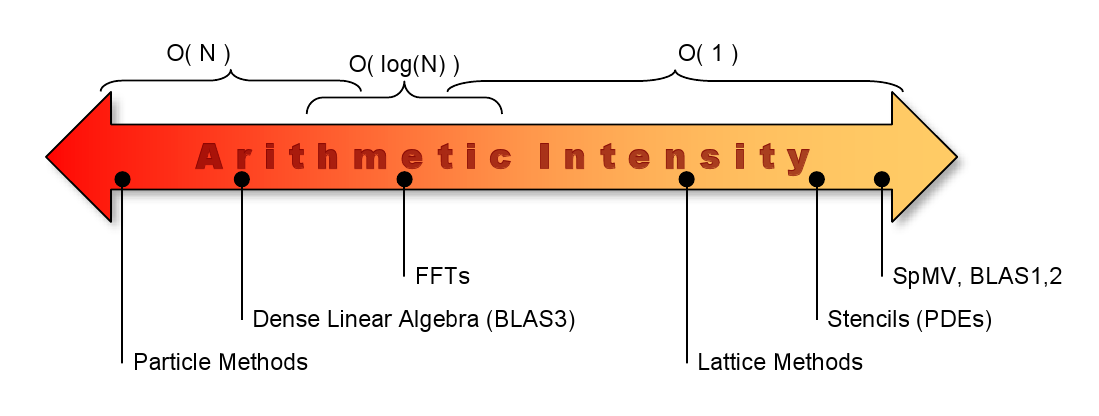
\includegraphics[width=0.95\textwidth]{figures/OlikerArithmeticIntensity.png} \\
    $\leftarrow$ Look at FLOPs \hspace{3cm} Look at Mem-BW $\rightarrow$
   \end{center}

\end{frame}





%%%%%%% GPUs: Disillusion %%%%%%%



\begin{frame}[fragile]
\frametitle{GPUs: Disillusion}
 \begin{block}{Computing Architecture Schematic}
  \begin{center}
   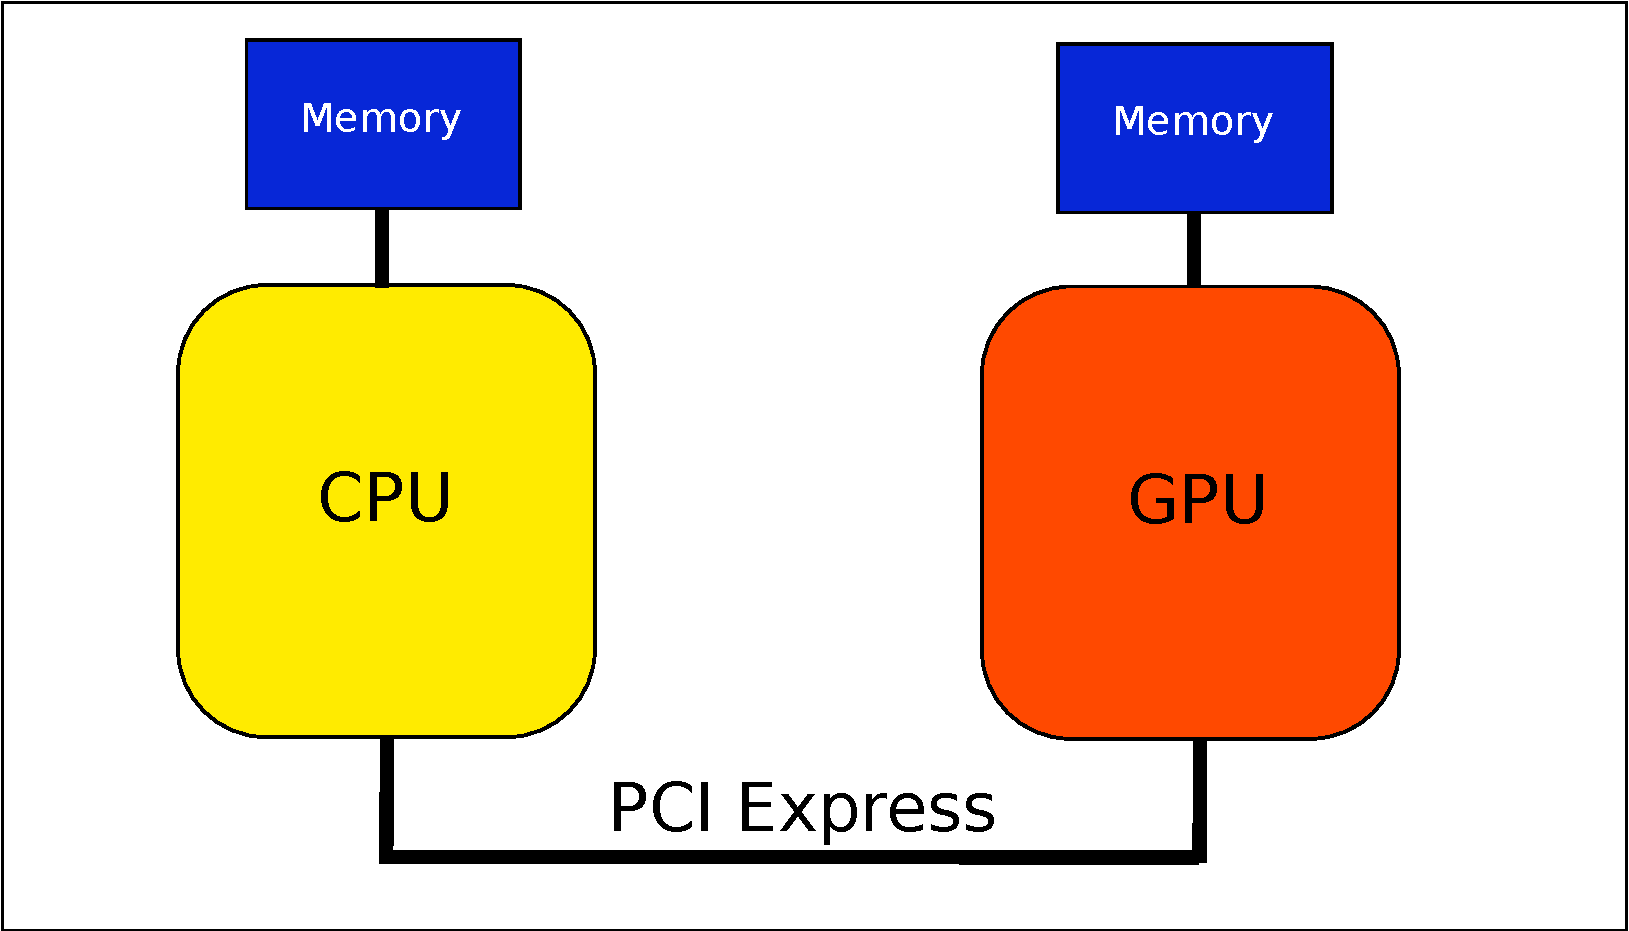
\includegraphics[width=0.8\textwidth]{figures/cpu-gpu-coarse.pdf}
  \end{center}

 
 \begin{itemize}
  \item \vspace*{1.03cm}
 \end{itemize}
 \end{block}

\end{frame}

\begin{frame}[fragile]
\frametitle{GPUs: Disillusion}
 \begin{block}{Computing Architecture Schematic}
  \begin{center}
   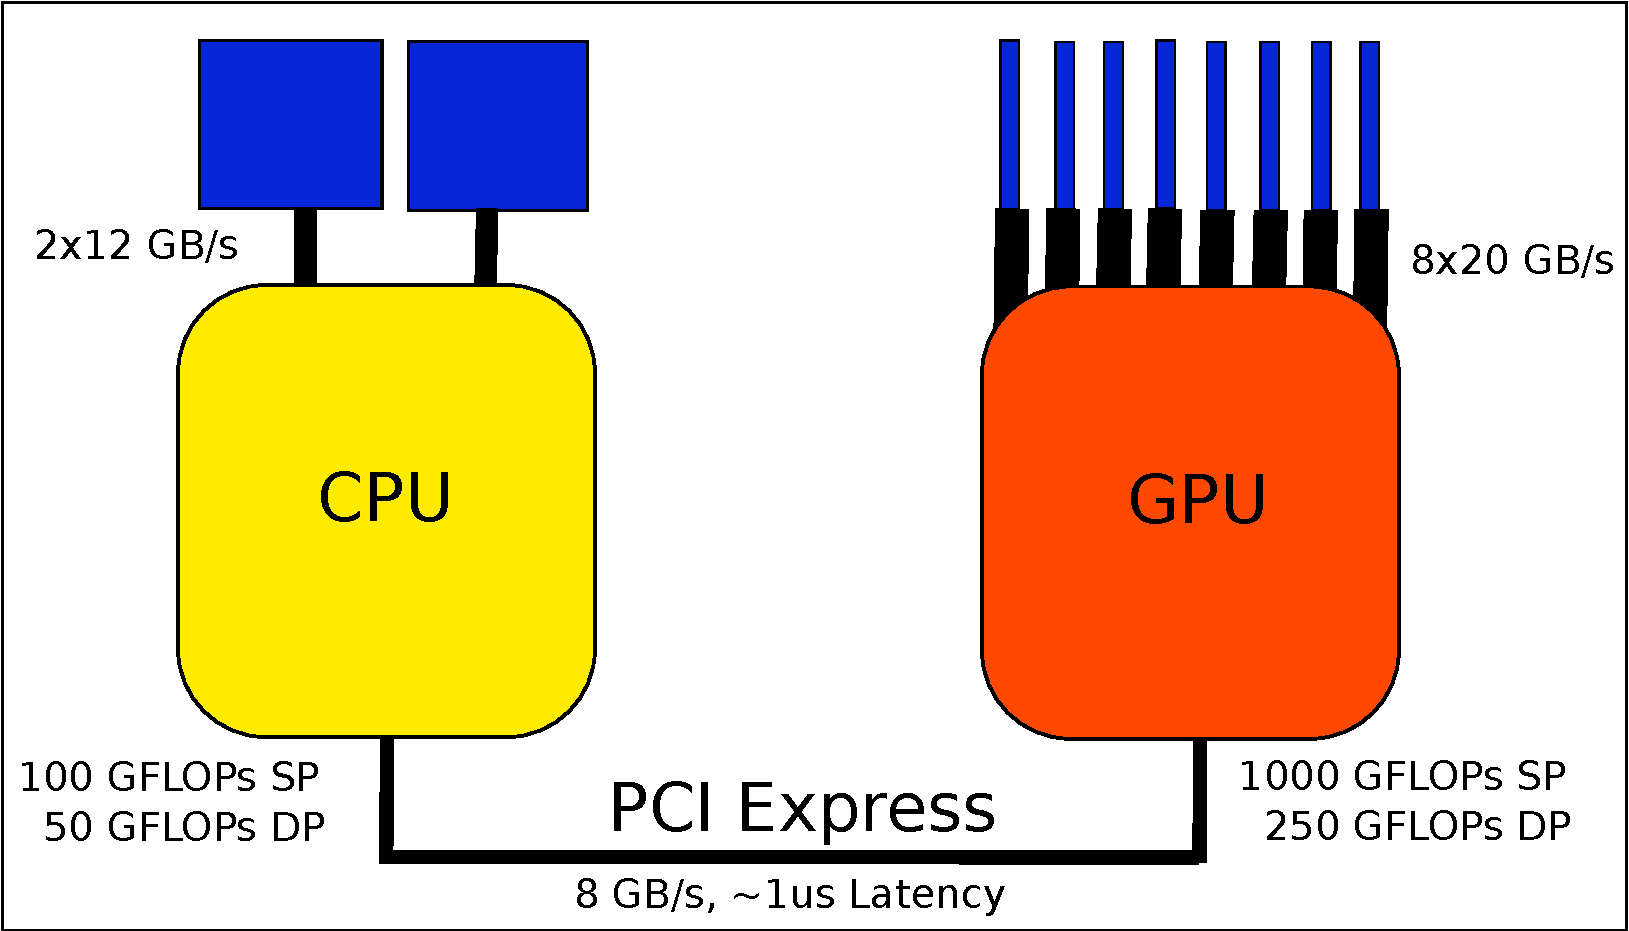
\includegraphics[width=0.8\textwidth]{figures/cpu-gpu-detail.pdf}
  \end{center}

 \begin{itemize}
  \item Good for large FLOP-intensive tasks, high memory bandwidth
  \item PCI-Express can be a bottleneck
  \item $\gg 10$-fold speedups (usually) not backed by hardware
 \end{itemize}
 \end{block}

\end{frame}


\begin{frame}{PETSc}
   \begin{center} (applet on architecture trends) \\[1em]
       {\footnotesize \url{http://www.eecs.berkeley.edu/~rcs/research/interactive\_latency.html}}
    \end{center}
\end{frame}





\begin{frame}{GPU Programming Approaches}
 
  \begin{block}{CUDA}
   \begin{itemize}
   \item Almost no additional code required
   \item Vendor-lock
   \item Relies on \lstinline|nvcc| being available
  \end{itemize}

  \end{block}

  \begin{block}{OpenCL}
  \begin{itemize}
   \item Additional boilerplate code required (low-level API)
   \item Broad hardware support (separate SDKs)
   \item No more development effort from NVIDIA
  \end{itemize}
  \end{block}

  \begin{block}{Directives}
   \begin{itemize}
    \item Annotate existing code with OpenMP-style Pragmas
    \item OpenACC and others
   \end{itemize}

  \end{block}

\end{frame}


\begin{frame}[fragile]{PETSc GPU Support}
 
  \begin{block}{NVIDIA Cusp/Thrust/CUSPARSE}
   \begin{itemize}
   \item Compile PETSc with CUDA support
   \item Use command line options to enable types, e.g.
    \begin{lstlisting}
 -vec_type cusp -mat_type aijcusp
    \end{lstlisting}
  \end{itemize}
  \end{block}

  \begin{block}{ViennaCL (OpenCL)}
  \begin{itemize}
   \item Compile PETSc with OpenCL support
   \item Use command line options to enable types, e.g.
    \begin{lstlisting}
 -vec_type viennacl -mat_type aijviennacl
    \end{lstlisting}
   \item Used for subsequent benchmarks
  \end{itemize}
  \end{block}

 \begin{center} No change in application code required! \end{center}
                                                        
\end{frame}


%%%% Which GPU is right for me?
\begin{frame}{Which Accelerator is Right for Me?}
 
  \begin{block}{Available Accelerators (Rough Sketch)}

   \begin{center}
    \begin{tabular}{|l|c|c|c|c|c|}
     \hline
      Name             & TFLOP/s & RAM (GB) & GB/s & TDP & Price \\
     \hline
     NVIDIA GTX 580    & 1.5/$\sim$0.2 & 1.5-3.0 & 192 & 244 & \$500   \\
     NVIDIA GTX Titan  & 4.5/1.3  & 6.0     & 288 & 250 & \$$\sim$1k \\
     NVIDIA Tesla 2050 & 1.3/0.5  & 3.0-6.0 & 150 & 225 & \$$\sim$2k \\
     NVIDIA K20        & 3.5/1.2  & 5.0     & 200 & 220 & \$$\sim$3k \\
     \hline
     AMD HD 7970       & 3.5/$\sim$0.9 & 3.0-6.0 & 264 & 250 & \$550 \\
     AMD FirePro W9k   & 4.0/1.0  & 6.0     & 264 & 274 & \$$\sim$3k \\
     \hline
     Intel Xeon Phi    & $\sim$2.0/$\sim$1.0 & 8 & 320 & 225 & \$$\sim$3k \\
     \hline
     \hline
     Intel Xeon E5-264x  & 0.2/0.1  & $\sim$64 & $\sim$48 & 100 & \$$\sim$1k \\
     \hline
   \end{tabular}
   \end{center}
  \end{block}

  %\visible<2>{
  \begin{block}{PETSc Considerations}
   \begin{itemize}
    \item Single precision performance doesn't matter
    \item Essentially all kernels memory bandwidth limited
    \item Memory access patterns rather irregular
   \end{itemize}
  \end{block}
  %}

\end{frame}






% \begin{frame}{Benchmarks}
%   \begin{center}
%    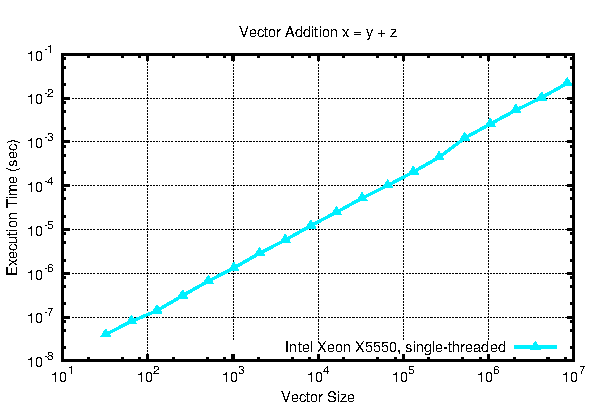
\includegraphics[width=0.95\textwidth]{figures/vector-timings-1}
%   \end{center}
% \end{frame}
% 
% \begin{frame}{Benchmarks}
%   \begin{center}
%    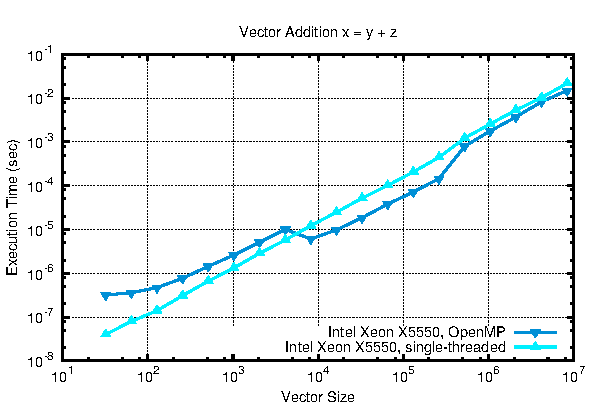
\includegraphics[width=0.95\textwidth]{figures/vector-timings-2}
%   \end{center}
% \end{frame}
% 
% \begin{frame}{Benchmarks}
%   \begin{center}
%    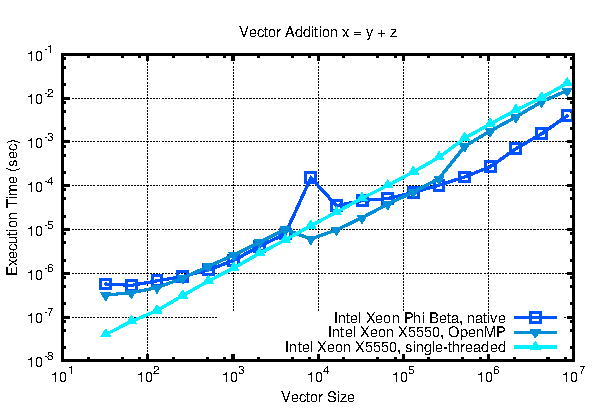
\includegraphics[width=0.95\textwidth]{figures/vector-timings-3}
%   \end{center}
% \end{frame}
% 
% \begin{frame}{Benchmarks}
%   \begin{center}
%    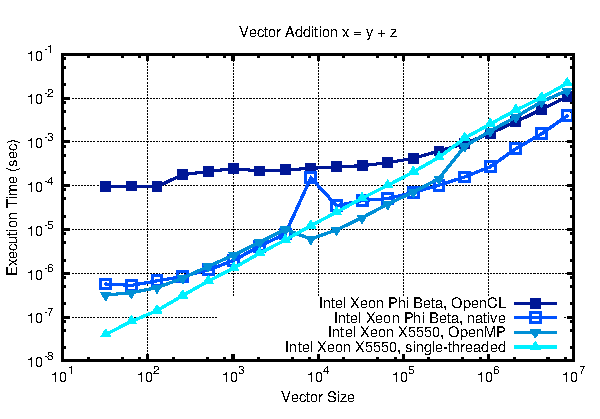
\includegraphics[width=0.95\textwidth]{figures/vector-timings-4}
%   \end{center}
% \end{frame}
% 
% \begin{frame}{Benchmarks}
%   \begin{center}
%    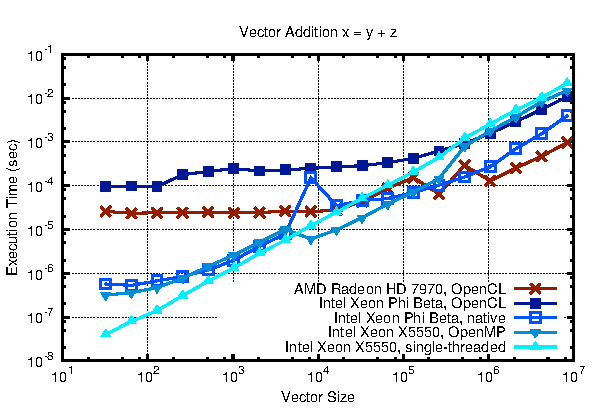
\includegraphics[width=0.95\textwidth]{figures/vector-timings-5}
%   \end{center}
% \end{frame}
% 
% \begin{frame}{Benchmarks}
%   \begin{center}
%    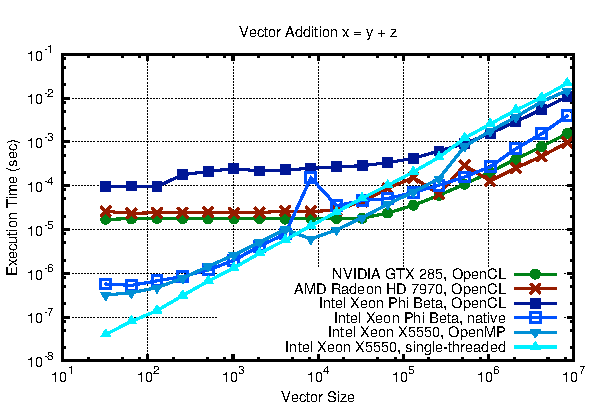
\includegraphics[width=0.95\textwidth]{figures/vector-timings-6}
%   \end{center}
% \end{frame}

\begin{frame}{Benchmarks}
  \begin{center}
   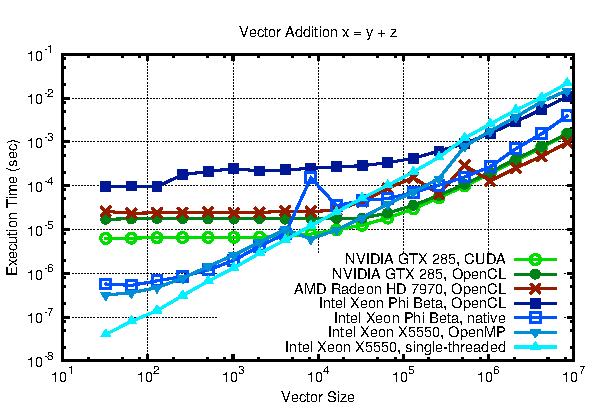
\includegraphics[width=0.95\textwidth]{figures/vector-timings-7}
  \end{center}
\end{frame}




% \begin{frame}{Benchmarks}
%   \begin{center}
%    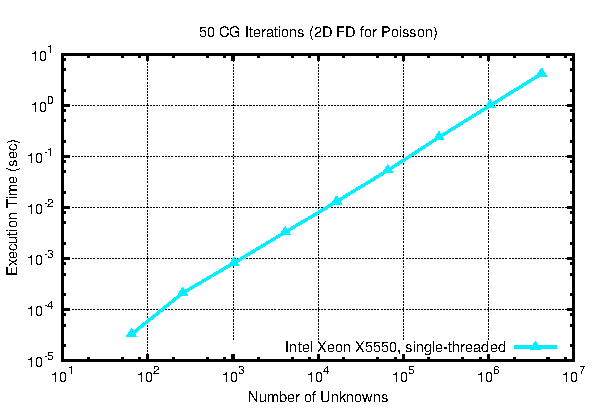
\includegraphics[width=0.95\textwidth]{figures/cg-timings-1}
%   \end{center}
% \end{frame}
% 
% \begin{frame}{Benchmarks}
%   \begin{center}
%    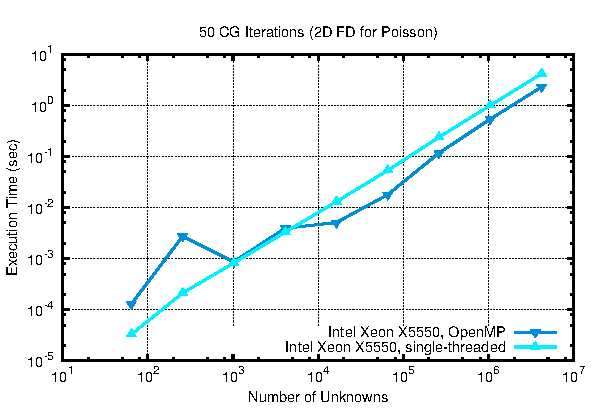
\includegraphics[width=0.95\textwidth]{figures/cg-timings-2}
%   \end{center}
% \end{frame}
% 
% \begin{frame}{Benchmarks}
%   \begin{center}
%    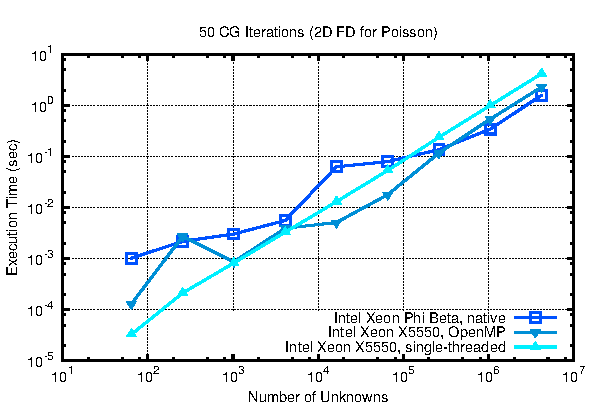
\includegraphics[width=0.95\textwidth]{figures/cg-timings-3}
%   \end{center}
% \end{frame}
% 
% \begin{frame}{Benchmarks}
%   \begin{center}
%    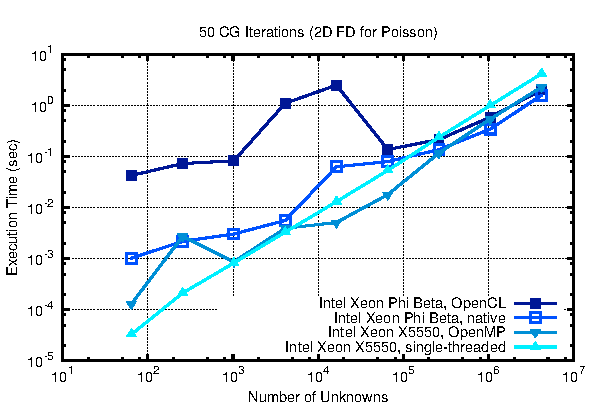
\includegraphics[width=0.95\textwidth]{figures/cg-timings-4}
%   \end{center}
% \end{frame}
% 
% \begin{frame}{Benchmarks}
%   \begin{center}
%    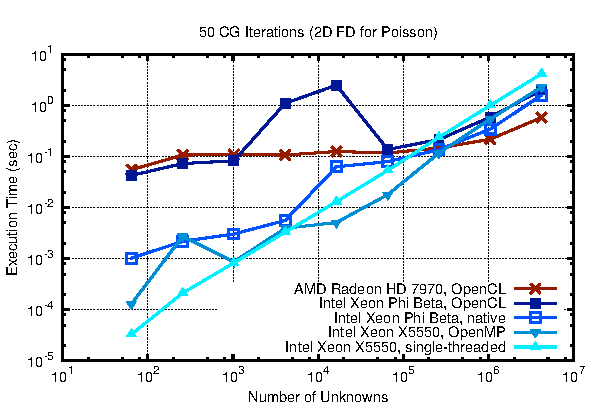
\includegraphics[width=0.95\textwidth]{figures/cg-timings-5}
%   \end{center}
% \end{frame}
% 
% \begin{frame}{Benchmarks}
%   \begin{center}
%    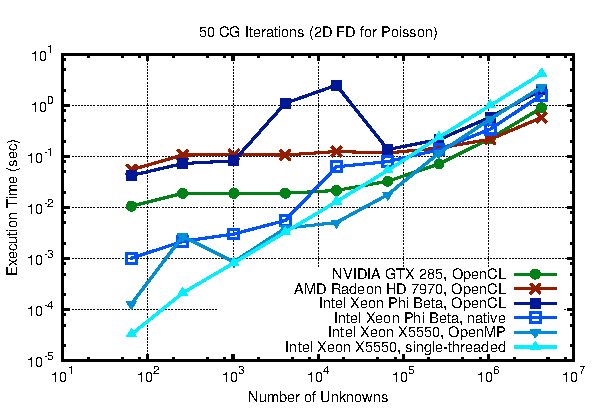
\includegraphics[width=0.95\textwidth]{figures/cg-timings-6}
%   \end{center}
% \end{frame}

\begin{frame}{Benchmarks}
  \begin{center}
   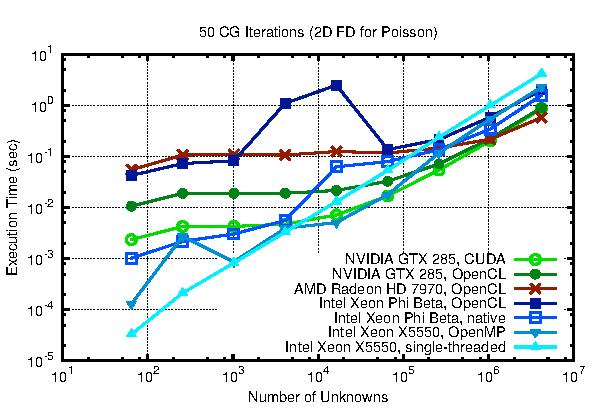
\includegraphics[width=0.95\textwidth]{figures/cg-timings-7}
  \end{center}
\end{frame}





%%%% Conclusion


\section{Conclusion}
\begin{frame}{End of Day 1}
 
 \begin{block}{PETSc can help You}
  \begin{itemize}
   \item solve algebraic and DAE problems in your application area
   \item rapidly develop efficient parallel code, can start from examples
   \item develop new solution methods and data structures
   \item debug and analyze performance
   \item advice on software design, solution algorithms, and performance
   \item \centering \texttt{petsc-\{users,dev,maint\}@mcs.anl.gov}

  \end{itemize}
 \end{block}

 \begin{block}{You can help PETSc}
  \begin{itemize}
   \item report bugs and inconsistencies, or if you think there is a better way
   \item tell us if the documentation is inconsistent or unclear
   \item consider developing new algebraic methods as plugins, contribute if your idea works
  \end{itemize}
 \end{block}

\end{frame}
